\documentclass{article}

\usepackage{fix-cm}
\usepackage[a0paper,portrait,margin=24mm]{geometry}
\usepackage{fontspec}
\usepackage{amsmath}
\usepackage{unicode-math}
\usepackage{array}
\usepackage{booktabs}
\usepackage{enumitem}
\usepackage{microtype}
\usepackage{ragged2e}
\usepackage{graphicx}
\usepackage[most]{tcolorbox}
\usepackage{tikz}
\usetikzlibrary{arrows.meta,calc,positioning,shapes.geometric}
\graphicspath{{./}}

\IfFontExistsTF{TeX Gyre Heros}{
  \setmainfont{TeX Gyre Heros}
}{
  \setmainfont{Latin Modern Sans}
}
\setmathfont{latinmodern-math.otf}
\renewcommand{\familydefault}{\sfdefault}

\definecolor{PosterInk}{HTML}{1B2430}
\definecolor{PosterMuted}{HTML}{56616F}
\definecolor{PosterPrimary}{HTML}{123B5D}
\definecolor{PosterAccent}{HTML}{C56A3A}
\definecolor{PosterTeal}{HTML}{237A80}
\definecolor{PosterSoft}{HTML}{F5F7FA}
\definecolor{PosterPanel}{HTML}{FFFFFF}
\definecolor{PosterRule}{HTML}{CBD5E1}
\definecolor{PosterTint}{HTML}{EAF2F7}
\definecolor{PosterWarmTint}{HTML}{FFF7ED}
\definecolor{PosterFuture}{HTML}{F1F4F7}

\pagestyle{empty}
\setlength{\parindent}{0pt}
\setlength{\parskip}{0.24em}
\setlist[itemize]{leftmargin=0.95em,itemsep=0.07em,topsep=0.08em}
\setlist[enumerate]{leftmargin=1.0em,itemsep=0.07em,topsep=0.08em}
\AtBeginDocument{\fontsize{17.8}{21.5}\selectfont\color{PosterInk}\justifying}

\newcommand{\PosterTitle}[1]{{\fontsize{45}{49}\selectfont\bfseries #1\par}}
\newcommand{\PosterSubtitle}[1]{{\fontsize{18.5}{23}\selectfont #1\par}}
\newcommand{\PosterMeta}[1]{{\fontsize{16.5}{20}\selectfont #1\par}}
\newcommand{\SmallNote}[1]{{\fontsize{12.5}{15}\selectfont\color{PosterMuted} #1}}
\newcommand{\PosterCaption}[1]{\par{\fontsize{9.8}{12}\selectfont\color{PosterMuted}\RaggedRight #1\par}}
\newcommand{\PosterReferenceText}[1]{{\fontsize{11.4}{13.5}\selectfont\color{PosterMuted}\RaggedRight #1\par}}
\newcommand{\Chip}[2][PosterTint]{%
  \tikz[baseline=(txt.base)]\node[
    fill=#1,
    draw=PosterRule,
    rounded corners=2.2mm,
    inner xsep=2.4mm,
    inner ysep=1.1mm
  ] (txt) {\fontsize{10.5}{12.5}\selectfont\bfseries\color{PosterPrimary} #2};%
}
\newcommand{\WarmChip}[1]{\Chip[PosterWarmTint]{#1}}
\newcommand{\FutureChip}[1]{\Chip[PosterFuture]{#1}}
\newcommand{\VarLine}[2]{\textbf{#1} & #2\\}
\newcommand{\StepLine}[1]{\tikz[baseline=-0.5ex]\node[circle,fill=PosterPrimary,inner sep=1.5pt]{};~#1\par}

\newtcolorbox{PosterBox}[1]{
  enhanced,
  colback=PosterPanel,
  colframe=PosterRule,
  boxrule=1.0pt,
  arc=2.4mm,
  left=6mm,
  right=6mm,
  top=7.5mm,
  bottom=4.5mm,
  before skip=0mm,
  after skip=4.7mm,
  title={#1},
  fonttitle=\fontsize{20.5}{24.5}\selectfont\bfseries,
  coltitle=white,
  boxed title style={
    colback=PosterPrimary,
    colframe=PosterPrimary,
    arc=1.8mm,
    left=4.4mm,
    right=4.4mm,
    top=1.6mm,
    bottom=1.6mm
  },
  attach boxed title to top left={xshift=5mm,yshift=-3.2mm}
}

\newtcolorbox{WidePosterBox}[1]{
  enhanced,
  colback=PosterPanel,
  colframe=PosterRule,
  boxrule=1.0pt,
  arc=2.4mm,
  left=6mm,
  right=6mm,
  top=7.5mm,
  bottom=4.5mm,
  before skip=0mm,
  after skip=4.7mm,
  title={#1},
  fonttitle=\fontsize{20.5}{24.5}\selectfont\bfseries,
  coltitle=white,
  boxed title style={
    colback=PosterPrimary,
    colframe=PosterPrimary,
    arc=1.8mm,
    left=4.4mm,
    right=4.4mm,
    top=1.6mm,
    bottom=1.6mm
  },
  attach boxed title to top left={xshift=5mm,yshift=-3.2mm}
}

\newcommand{\StatusStrip}{%
  
\begin{tikzpicture}[
    x=1mm,y=1mm,
    status/.style={draw=PosterRule,rounded corners=2mm,minimum height=10mm,inner xsep=2.2mm,align=center,font=\fontsize{10.5}{12}\selectfont\bfseries}
  ]
    \node[status,fill=PosterTint,text=PosterPrimary] at (22,0) {IMPLEMENTED};
    \node[status,fill=PosterTint,text=PosterPrimary] at (70,0) {VERIFIED};
    \node[status,fill=PosterWarmTint,text=PosterAccent] at (120,0) {CHARACTERISED};
    \node[status,fill=PosterTint,text=PosterTeal] at (174,0) {DEMONSTRATED};
    \node[status,fill=PosterFuture,text=PosterMuted] at (224,0) {FUTURE};
  \end{tikzpicture}
}

\newcommand{\FrameworkGraphic}{%
  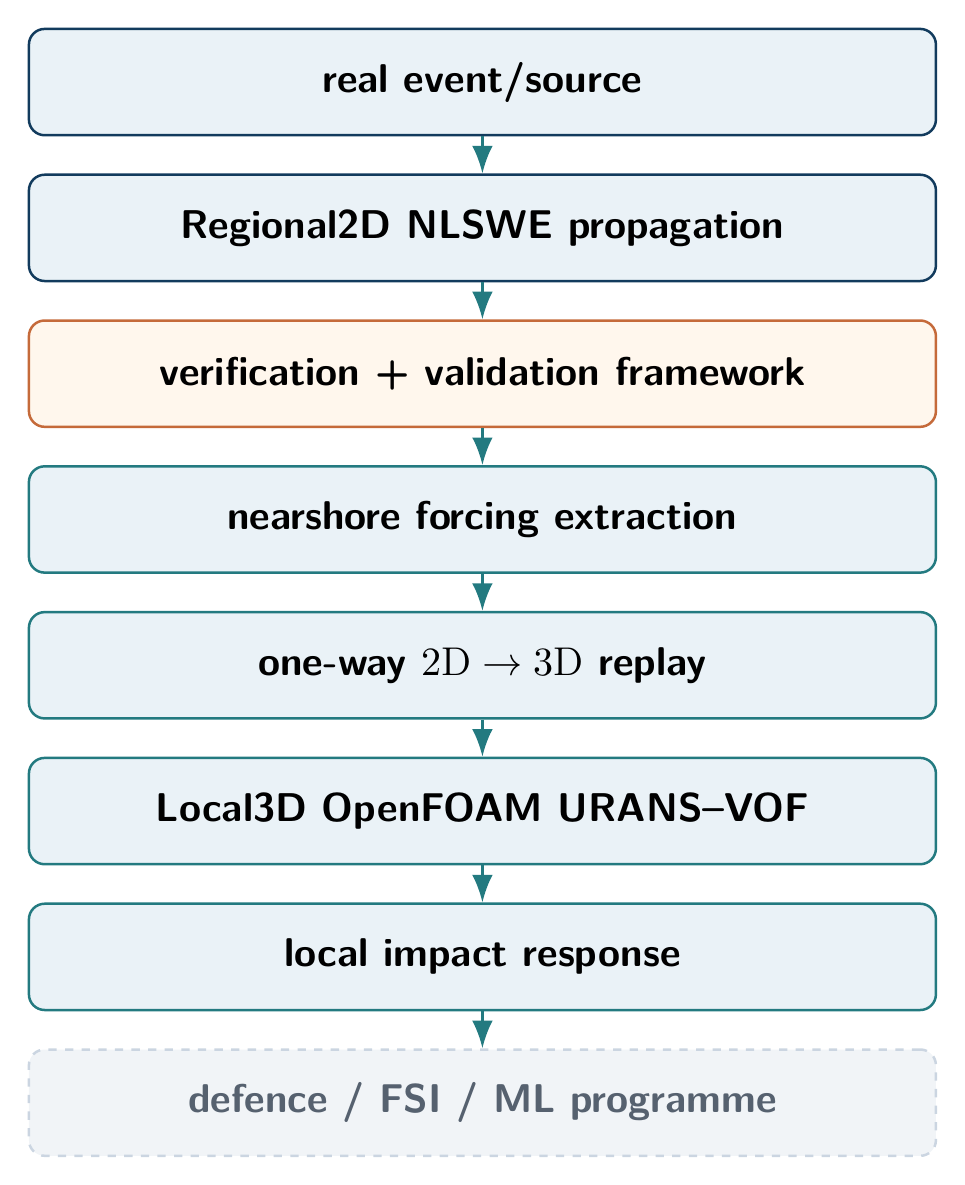
\begin{tikzpicture}[
    node distance=4.7mm,
    stage/.style={
      draw=PosterPrimary,
      fill=PosterTint,
      rounded corners=2mm,
      line width=0.9pt,
      minimum width=0.95\linewidth,
      minimum height=13.5mm,
      inner sep=2.2mm,
      align=center,
      font=\fontsize{14.5}{17}\selectfont\bfseries
    },
    future/.style={
      draw=PosterRule,
      fill=PosterFuture,
      rounded corners=2mm,
      dashed,
      line width=0.9pt,
      minimum width=0.95\linewidth,
      minimum height=13.5mm,
      inner sep=2.2mm,
      align=center,
      font=\fontsize{14.5}{17}\selectfont\bfseries\color{PosterMuted}
    },
    arrow/.style={-{Latex[length=3.5mm]},line width=1.0pt,draw=PosterTeal}
  ]
    \node[stage] (event) {real event/source};
    \node[stage,below=of event] (regional) {Regional2D NLSWE propagation};
    \node[stage,below=of regional,draw=PosterAccent,fill=PosterWarmTint] (cred) {verification + validation framework};
    \node[stage,below=of cred,draw=PosterTeal,fill=PosterTint] (forcing) {nearshore forcing extraction};
    \node[stage,below=of forcing,draw=PosterTeal,fill=PosterTint] (replay) {one-way \(2\mathrm{D}\rightarrow3\mathrm{D}\) replay};
    \node[stage,below=of replay,draw=PosterTeal,fill=PosterTint] (local) {Local3D OpenFOAM URANS--VOF};
    \node[stage,below=of local,draw=PosterTeal,fill=PosterTint] (impact) {local impact response};
    \node[future,below=of impact] (future) {defence / FSI / ML programme};
    \foreach \a/\b in {event/regional,regional/cred,cred/forcing,forcing/replay,replay/local,local/impact,impact/future}
      \draw[arrow] (\a) -- (\b);
  \end{tikzpicture}
}

\newcommand{\RegionalAlgorithm}{%
  \StepLine{event + terrain state}
  \StepLine{wet/dry classification}
  \StepLine{limited-linear \(\eta,u,v\) reconstruction}
  \StepLine{hydrostatic reconstruction}
  \StepLine{Rusanov numerical face flux}
  \StepLine{bed, Manning and boundary sources}
  \StepLine{CFL-controlled timestep}
  \StepLine{SSPRK3 update}
  \StepLine{positivity, diagnostics and output}
}

\newcommand{\LocalAlgorithm}{%
  \StepLine{regional replay boundary data}
  \StepLine{\(\eta,q_n,q_t\) inlet reconstruction}
  \StepLine{\(\alpha_{\mathrm{water}} + \mathbf U\) boundary state}
  \StepLine{OpenFOAM incompressible two-phase URANS--VOF}
  \StepLine{pressure / velocity coupling}
  \StepLine{VOF interface transport}
  \StepLine{\(k\)--\(\omega\) SST turbulence}
  \StepLine{Courant and interface-Courant control}
  \StepLine{fields, probes, \(F(t)\), \(M(t)\)}
}

\begin{document}

\begin{tcolorbox}[
  enhanced,
  colback=PosterPrimary,
  colframe=PosterPrimary,
  arc=3mm,
  boxrule=0pt,
  left=12mm,
  right=12mm,
  top=8mm,
  bottom=8mm
]
  {\color{white}
  \PosterTitle{A Coupled 2D NLSWE Regional-Propagation and\\
  3D URANS--VOF Coastal-Impact Framework for Reconstructing the\\
  2011 Tōhoku Tsunami}
  \vspace{2mm}
  \PosterSubtitle{Research snapshot from an ongoing framework-development programme. The work presented establishes and verifies the computational foundation for future historical validation, coastal-impact studies and tsunami-defence assessment; it does not claim a fully validated reconstruction of the 2011 event.}
  \vspace{2.2mm}
  \PosterMeta{Rhyen Jivan \quad | \quad Summer Studentship Project}
  }
\end{tcolorbox}

\vspace{3.5mm}

\noindent
\begin{minipage}[t]{0.652\textwidth}
  \vspace{0pt}
  \begin{WidePosterBox}{Real-event reconstruction}
    \begin{minipage}[t]{0.43\linewidth}
      \vspace{0pt}
      \centering
      \includegraphics[width=0.98\linewidth,height=188mm,keepaspectratio]{\detokenize{Studentship - Figures.png}}
      \PosterCaption{\textbf{Figure A.} Regional context of the 2011 Tōhoku earthquake and Kamaishi Regional2D corridor. Base map adapted from Encyclopaedia Britannica; corridor and Kamaishi annotations added for this study.}
    \end{minipage}
    \hfill
    \begin{minipage}[t]{0.53\linewidth}
      \vspace{0pt}
      {\fontsize{22}{26}\selectfont\bfseries\color{PosterPrimary} Kamaishi target case\par}
      \vspace{1.5mm}
      Kamaishi is used as the target coastal case study for reconstructing source-to-coast tsunami propagation from the 2011 Tōhoku event. The Regional2D corridor passes through the event reference and carries the wave toward the selected wet nearshore interface.

      \vspace{5mm}
      \StatusStrip

      \vspace{4mm}
      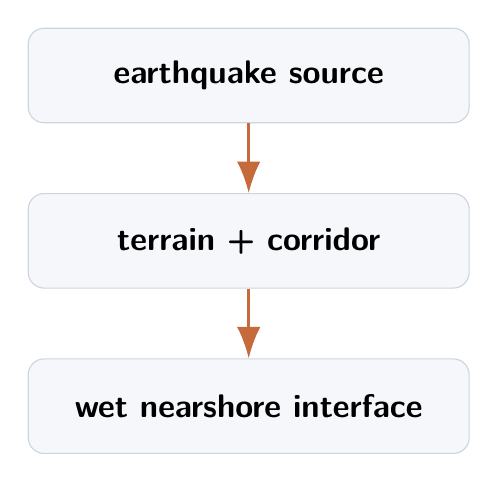
\begin{tikzpicture}[
        x=1mm,y=1mm,
        node/.style={draw=PosterRule,fill=PosterSoft,rounded corners=2mm,minimum width=56mm,minimum height=12mm,align=center,font=\fontsize{11.8}{14}\selectfont\bfseries},
        arrow/.style={-{Latex[length=4mm]},line width=1.0pt,draw=PosterAccent}
      ]
        \node[node] (source) at (31,52) {earthquake source};
        \node[node] (terrain) at (31,31) {terrain + corridor};
        \node[node] (interface) at (31,10) {wet nearshore interface};
        \draw[arrow] (source) -- (terrain);
        \draw[arrow] (terrain) -- (interface);
      \end{tikzpicture}

      \vspace{2mm}
      \SmallNote{The real-event panel is organised as a visual sequence: regional context first, then oblique corridor geometry and the longitudinal bathymetric profile.}
    \end{minipage}

    \vspace{3.5mm}
    \noindent
    \begin{minipage}[t]{0.49\linewidth}
      \vspace{0pt}
      \centering
      \includegraphics[width=\linewidth,height=86mm,keepaspectratio]{\detokenize{Studentship - Figures (1).png}}
      \PosterCaption{\textbf{Figure B.} Oblique bathymetry and topography of the Kamaishi Regional2D corridor. NOAA/NCEI ETOPO 2022, EGM2008; prepared in QGIS/GDAL and rendered in Blender 5.2 EEVEE with \(4\times\) vertical exaggeration.}
    \end{minipage}
    \hfill
    \begin{minipage}[t]{0.49\linewidth}
      \vspace{0pt}
      \centering
      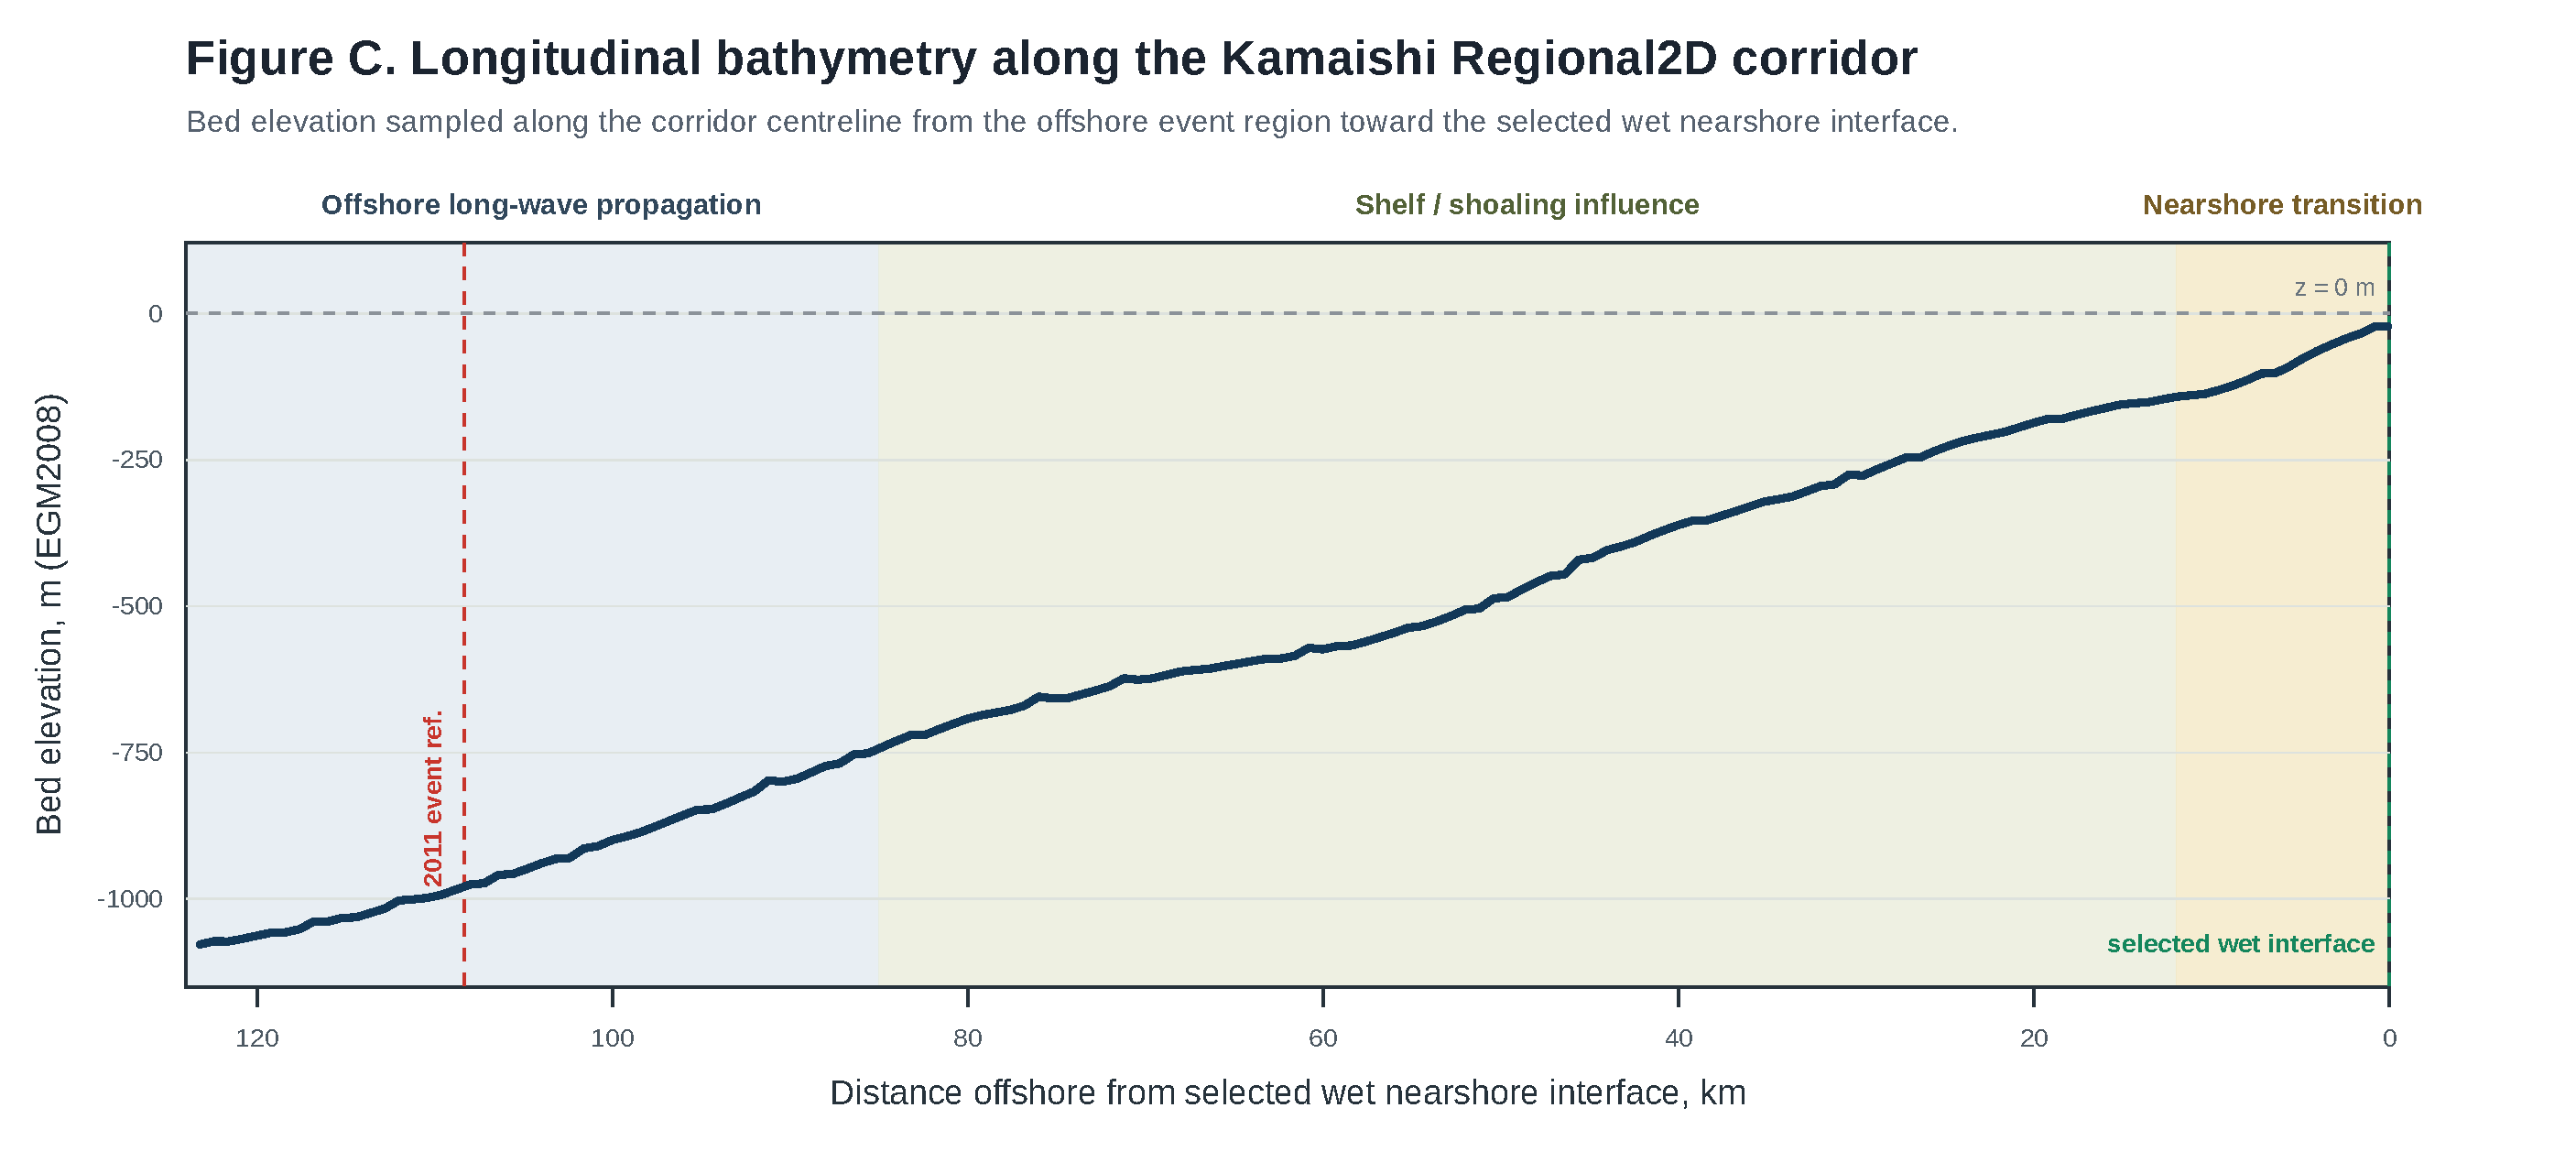
\includegraphics[width=\linewidth,height=86mm,keepaspectratio]{figure_C_longitudinal_bathymetry_poster_clean.pdf}
      \PosterCaption{\textbf{Figure C.} Longitudinal bathymetry along the Kamaishi Regional2D corridor. Profile sampled along the accepted corridor centreline; bed elevation referenced to EGM2008.}
    \end{minipage}
  \end{WidePosterBox}
\end{minipage}
\hfill
\begin{minipage}[t]{0.328\textwidth}
  \vspace{0pt}
  \begin{PosterBox}{Why this matters}
    Defence assessment needs local loading and impact physics while preserving the link to the real tsunami source. Full source-to-coast 3D simulation is impractical, but purely depth-averaged modelling cannot resolve vertical impact, free-surface deformation or structure loading. Hybrid modelling bridges those scales.
  \end{PosterBox}

  \begin{PosterBox}{Aim and objectives}
    \textbf{Aim:} Establish a computational framework for reconstructing and validating real tsunami events, then reuse validated event forcing for Local3D coastal-impact and tsunami-defence studies.

    \begin{enumerate}
      \item Reconstruct the 2011 Tōhoku source using real event and terrain data.
      \item Propagate the event through a verified Regional2D NLSWE corridor.
      \item Establish observation-based historical-validation methodology.
      \item Demonstrate one-way transfer into a Local3D URANS--VOF impact model.
      \item Define response quantities for defence, resilience and optimisation.
    \end{enumerate}
  \end{PosterBox}

  \begin{PosterBox}{Hybrid framework overview}
    \centering
    \FrameworkGraphic
    \PosterCaption{System architecture only: implemented and verified modelling stages are separated from planned defence, FSI and data-driven extensions.}
  \end{PosterBox}
\end{minipage}

\vspace{4mm}

\noindent
\begin{minipage}[t]{0.318\textwidth}
  \vspace{0pt}
  \begin{PosterBox}{Variables \& quantities of interest}
    \SmallNote{\textbf{Solved / exported fields}}\par
    \vspace{1.5mm}
    \begin{tabular}{@{}p{0.18\linewidth}p{0.73\linewidth}@{}}
      \multicolumn{2}{@{}l}{\textbf{Regional propagation state}}\\
      \VarLine{\(\eta\)}{free-surface elevation}
      \VarLine{\(h\)}{water depth}
      \VarLine{\(q_x,q_y\)}{depth-integrated discharge}
      \VarLine{\(u,v\)}{depth-averaged velocity}
      \VarLine{\(b\)}{bed elevation / bathymetry}
      \VarLine{\(\Delta z_b\)}{coseismic bed displacement}
    \end{tabular}

    \vspace{3mm}
    \begin{tabular}{@{}p{0.20\linewidth}p{0.71\linewidth}@{}}
      \multicolumn{2}{@{}l}{\textbf{Local flow / material state}}\\
      \VarLine{\(\mathbf U\)}{3D velocity}
      \VarLine{\(p\)}{pressure}
      \VarLine{\(\alpha_{\mathrm{water}}\)}{water volume fraction}
      \VarLine{\(\rho,\mu,\mu_t\)}{mixture density and viscosities}
      \VarLine{\(k,\omega\)}{SST turbulence variables}
      \VarLine{\(Re,y^+\)}{diagnostic regime and wall resolution}
    \end{tabular}

    \vspace{3mm}
    \SmallNote{\textbf{Derived / future study metrics}}\par
    \vspace{1.5mm}
    \begin{tabular}{@{}p{0.23\linewidth}p{0.68\linewidth}@{}}
      \multicolumn{2}{@{}l}{\textbf{Loading \& interaction}}\\
      \VarLine{\(\tau_w\)}{wall shear stress}
      \VarLine{\(F(t),M(t)\)}{resultant force and moment}
      \VarLine{\(J\)}{force impulse}
      \VarLine{}{pressure loading; viscous traction}\\[1mm]
      \multicolumn{2}{@{}l}{\textbf{Coastal / defence response}}\\
      \VarLine{}{run-up; inundation depth}
      \VarLine{}{overtopping discharge / volume}
      \VarLine{}{transmission; momentum transmission}
      \VarLine{}{mechanical-energy transmission / dissipation}
    \end{tabular}

    \vspace{2mm}
    \SmallNote{Response metrics define the later defence-study vocabulary; they are not all validated 2011-event results.}
  \end{PosterBox}
\end{minipage}
\hfill
\begin{minipage}[t]{0.318\textwidth}
  \vspace{0pt}
  \begin{PosterBox}{Solution algorithms}
    \begin{minipage}[t]{0.48\linewidth}
      {\fontsize{19}{23}\selectfont\bfseries\color{PosterPrimary} Regional2D\par}
      \RegionalAlgorithm
    \end{minipage}
    \hfill
    \begin{minipage}[t]{0.48\linewidth}
      {\fontsize{19}{23}\selectfont\bfseries\color{PosterPrimary} Local3D: adopted backend\par}
      \LocalAlgorithm
    \end{minipage}

    \vspace{4mm}
    \begin{tcolorbox}[enhanced,colback=PosterSoft,colframe=PosterRule,boxrule=0.8pt,arc=2mm,left=3mm,right=3mm,top=2mm,bottom=2mm]
      {\fontsize{12.8}{15.5}\selectfont
      \textbf{Pseudocode strip.} For each regional step: reconstruct face states; apply hydrostatic treatment; compute fluxes and source terms; advance SSPRK3 stages; enforce admissibility; publish diagnostics. For each replay step: update mapped inlet forcing; advance OpenFOAM URANS--VOF state; monitor boundedness and Courant limits; extract free-surface and impact diagnostics.}
    \end{tcolorbox}

    \SmallNote{The repository configures and audits OpenFOAM Foundation 11; it does not reimplement OpenFOAM pressure-correction, VOF or turbulence internals.}
  \end{PosterBox}
\end{minipage}
\hfill
\begin{minipage}[t]{0.318\textwidth}
  \vspace{0pt}
  \begin{PosterBox}{Verification method}
    \textbf{Model / implementation consistency:} research formulation \(\rightarrow\) implementation traceability \(\rightarrow\) zero required mismatches.

    \vspace{2mm}
    \textbf{Controlled Regional verification:}
    \begin{itemize}
      \item manufactured solution \(\rightarrow\) \Chip{FIRST ORDER BASELINE VERIFIED}
      \item limited-linear reconstruction \(\rightarrow\) \Chip{SECOND ORDER LIMITED-LINEAR VERIFIED}
      \item smooth-wave benchmark: amplitude error reduced \(5.35\times\); phase-proxy error reduced \(17.43\times\).
    \end{itemize}

    \vspace{1mm}
    \textbf{Real-event numerical fidelity:}
    \begin{itemize}
      \item real-event refinement and projection-only diagnosis completed;
      \item terrain/source fidelity is the characterised dominant limitation;
      \item current real-event forcing is \textbf{BEST AVAILABLE -- NUMERICALLY UNCERTAIN}.
    \end{itemize}

    \vspace{1mm}
    \textbf{Hybrid / Local3D evidence:} forcing/replay consistency, boundary-reflection benchmark, VOF/runtime boundedness evidence, \(y^+\) wall-treatment checks, probes and force/moment extraction.
  \end{PosterBox}

  \begin{PosterBox}{Current achievements}
    \begin{itemize}
      \item Regional2D implementation traced consistently to the research formulation.
      \item First-order baseline and limited-linear second-order formulation formally verified.
      \item Real 2011 Tōhoku \(\rightarrow\) Kamaishi Regional2D reconstruction completed.
      \item Terrain/source fidelity characterised as the present real-event spatial limitation.
      \item One-way Regional2D\(\rightarrow\)Local3D replay framework implemented and demonstrated.
      \item Accepted no-defence and simple-rigid-barrier Local3D replay evidence includes free-surface/probe output and force/moment extraction.
      \item Historical observation catalogue and validation methodology established.
    \end{itemize}
  \end{PosterBox}
\end{minipage}

\vspace{3mm}

\noindent
\begin{minipage}[t]{0.49\textwidth}
  \vspace{0pt}
  \begin{PosterBox}{Validation framework}
    \begin{minipage}[t]{0.48\linewidth}
      \textbf{Observation targets}
      \begin{itemize}
        \item offshore/deep-ocean waveform;
        \item domain-compatible Kamaishi/offshore observations;
        \item run-up;
        \item inundation.
      \end{itemize}
    \end{minipage}
    \hfill
    \begin{minipage}[t]{0.48\linewidth}
      \textbf{Metrics}
      \begin{itemize}
        \item RMSE; MAE; Bias; correlation;
        \item peak-amplitude error;
        \item peak-time error.
      \end{itemize}
    \end{minipage}

    \vspace{2mm}
    \Chip{VALIDATION FRAMEWORK ESTABLISHED}\quad
    \WarmChip{0 DIRECT}\quad
    \WarmChip{1 PROXY}\quad
    \WarmChip{28 TARGET ONLY}

    \vspace{2mm}
    \SmallNote{Primary validation uses no arbitrary time shift or amplitude scaling. Direct collocated waveform validation is not yet complete.}
  \end{PosterBox}
\end{minipage}
\hfill
\begin{minipage}[t]{0.49\textwidth}
  \vspace{0pt}
  \begin{PosterBox}{Next steps}
    \begin{enumerate}
      \item Improve event/source and terrain fidelity, and refine or extend the validation domain where observation colocation requires it.
      \item Perform uncalibrated historical comparison, followed by documented calibration and holdout validation.
      \item Resolve current-generation Local3D VOF replay boundedness before adopting latest regional forcing for impact studies.
      \item Execute systematic no-defence / defence impact comparisons using agreed loading, overtopping, inundation and transmission metrics.
      \item Extend toward FSI, structural resilience, impact-response databases and future ML-based optimisation/design.
    \end{enumerate}
  \end{PosterBox}
\end{minipage}

\vfill
\begin{PosterBox}{References}
  \PosterReferenceText{%
  Encyclopaedia Britannica; Japan Earthquake and Tsunami of 2011; Encyclopaedia Britannica; n.d. \quad
  NOAA National Centers for Environmental Information; ETOPO 2022 15 Arc-Second Global Relief Model; NOAA/NCEI; 2022. \quad
  Fujii et al.; Tsunami Source of the 2011 off the Pacific Coast of Tohoku Earthquake; Earth, Planets and Space; 2011. \quad
  Mori, Takahashi and The 2011 Tohoku Earthquake Tsunami Joint Survey Group; Nationwide Post Event Survey and Analysis of the 2011 Tohoku Earthquake Tsunami; Coastal Engineering Journal; 2012. \quad
  Kurganov and Petrova; A Second-Order Well-Balanced Positivity Preserving Central-Upwind Scheme for the Saint-Venant System; Communications in Mathematical Sciences; 2007. \quad
  Hirt and Nichols; Volume of Fluid (VOF) Method for the Dynamics of Free Boundaries; Journal of Computational Physics; 1981. \quad
  Menter; Two-Equation Eddy-Viscosity Turbulence Models for Engineering Applications; AIAA Journal; 1994. \quad
  Fujima, Masamura and Goto; Development of the 2D/3D Hybrid Model for Tsunami Numerical Simulation; Coastal Engineering Journal; 2002. \quad
  Takase et al.; 2D--3D Hybrid Stabilized Finite Element Method for Tsunami Runup Simulations; Computational Mechanics; 2016. \quad
  Watanabe et al.; Validation of Tsunami Numerical Simulation Models for an Idealized Coastal Industrial Site; Coastal Engineering Journal; 2022.}
\end{PosterBox}

\end{document}
